\documentclass[../../ASSD_TP1_G7.tex]{subfiles}
\begin{document}
\chapter*{Ejercicios te\'oricos}


\section*{Ejercicio 9.1}
Llamando a $x(n)=X(nT)$ y $y(n)=Y(nT)$, se obtiene la siguiente ecuación en diferencias. 
\begin{equation}
y(n)=\frac{1}{2} x(n-2) + \alpha y(n-1) + \beta y(n-2)  
\end{equation}

\subsection*{a}
Siendo $\alpha = 1$ y $\beta = -\frac{1}{2}$ se simulo la respuesta al escalón y al impulso.


\begin{figure}[H]
\centering
\subcaptionbox{Respuesta al escalón\label{f:ejaesc}}
{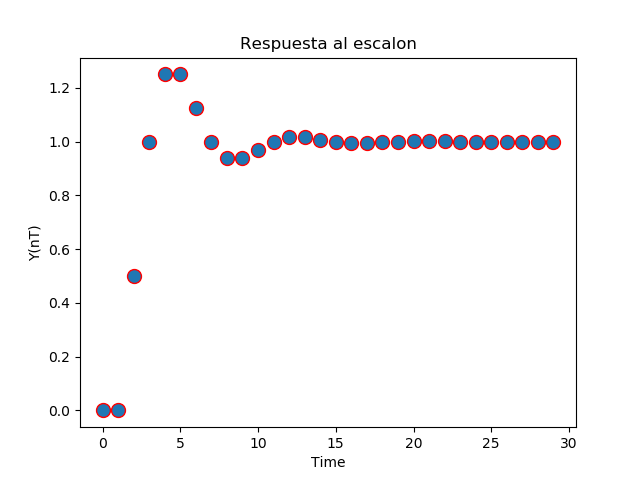
\includegraphics[width=0.45\textwidth]{figures/a-escalon.png}}
\subcaptionbox{Respuesta al impulso\label{f:ejaimp}}
{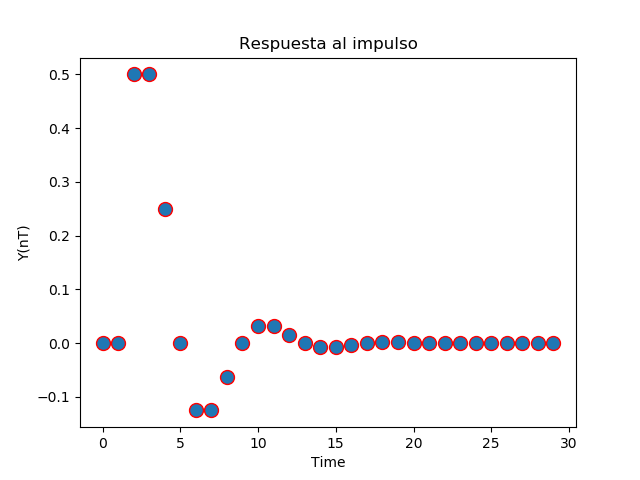
\includegraphics[width=0.45\textwidth]{figures/a-impulso.png}}
\caption{Gráficos de la simulación de las respuesta al impulso y al escalón}\label{f:eja}
\end{figure}



De la simulación se obtuvo que la frecuencia de oscilación en función de $nT$ es $f= \frac{1}{8}$.
\subsection*{b}
Siendo $\alpha = \frac{1}{2}$ y $\beta = -\frac{1}{8}$ se simulo la respuesta al escalón y al impulso.


\begin{figure}[H]
\centering
\subcaptionbox{Respuesta al escalón\label{f:ejbesc}}
{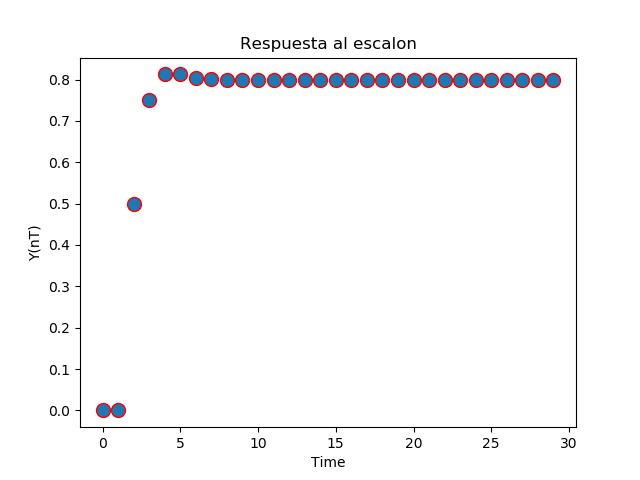
\includegraphics[width=0.45\textwidth]{figures/b-escalon.png}}
\subcaptionbox{Respuesta al impulso\label{f:ejbimp}}
{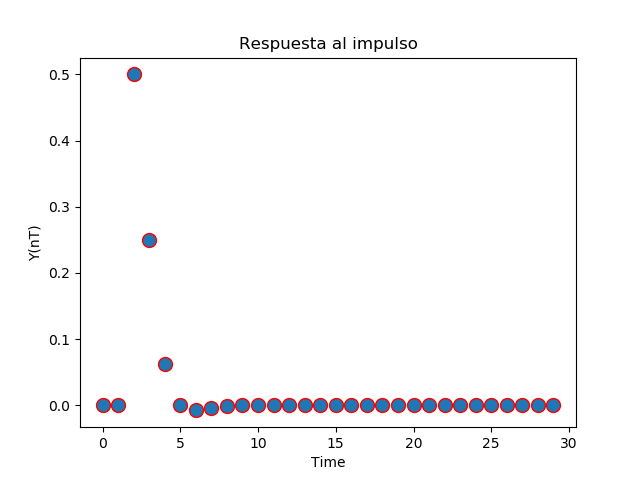
\includegraphics[width=0.45\textwidth]{figures/b-impulso.png}}
\caption{Gráficos de la simulación de las respuesta al impulso y al escalón}\label{f:ejb}
\end{figure}


\subsection*{c}
Siendo $\alpha = 1$ y $\beta = -\frac{1}{2}$ se simulo la respuesta al escalón y al impulso.


\begin{figure}[H]
\centering
\subcaptionbox{Respuesta al escalón\label{f:ejcesc}}
{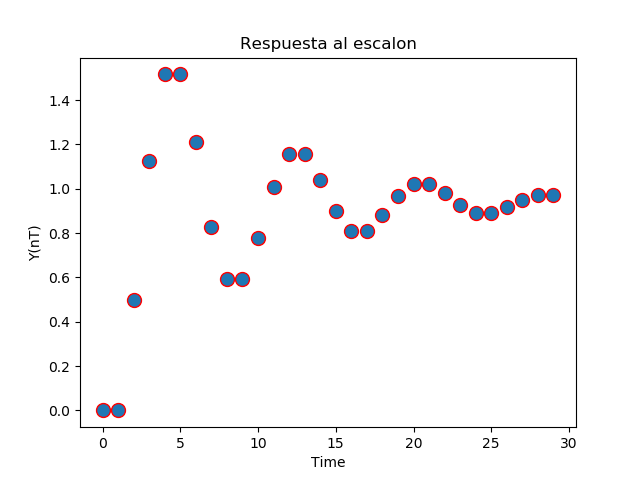
\includegraphics[width=0.45\textwidth]{figures/c-escalon.png}}
\subcaptionbox{Respuesta al impulso\label{f:ejcimp}}
{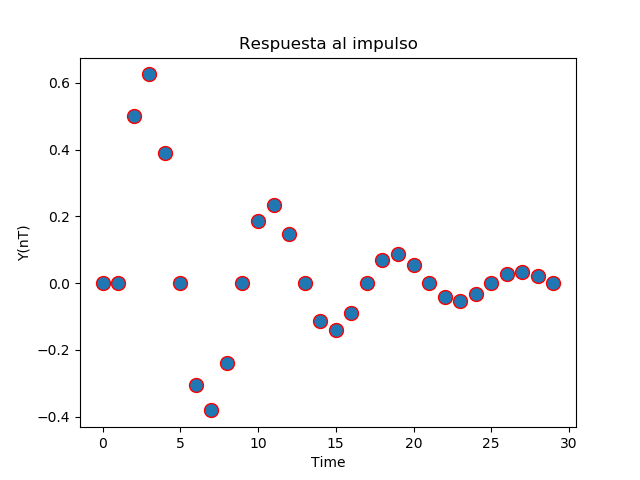
\includegraphics[width=0.45\textwidth]{figures/c-impulso.png}}
\caption{Gráficos de la simulación de las respuesta al impulso y al escalón}\label{f:ejc}
\end{figure}


De la simulación se obtuvo que la frecuencia de oscilación en función de $nT$ es $f= \frac{1}{7}$
\subsection*{Respuesta en frecuencia}
Para hallar el modulo de la respuesta en frecuencia, se ingreso al sistema con un seno de amplitud unitario y un tiempo mayor al del establecimiento, se midió el máximo de la se\~nal de entrada. Dicho proceso se repitió para distintas frecuencias entre 0 y $\frac{w_s}{2} $

\begin{figure}[H]
  \centering
   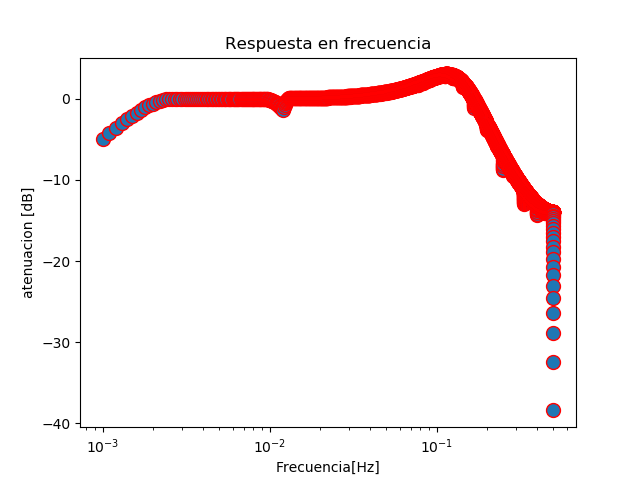
\includegraphics[width=0.9\textwidth]{figures/rtaFrec.png}
  \caption{Modulo de la respuesta en frecuencia simulada}
  \label{fig:rtaFrecFin}
\end{figure}
\subsection{Análisis de resultados}
Como se observa las respuesta del sistema, con los parámetros de los casos $a$ y $c$, corresponde a un sistema subamortiguado. En el caso $a$ corresponde a un sistema subamortiguado con un factor de amortiguamiento mayor que el caso $c$.
\par El caso de $c$ corresponde a un sistema críticamente amortiguado.






\section{Retardo de grupo}
El sistema propuesto: $y(n)=x(n)+2x(n-1)+3x(n-2)+4x(n-3)+3x(n-4)+2x(n-5)+x(n-6)$  esta representado por una ecuaci\'{o}n de diferencias lineales con coeficientes constantes por lo que fácilmente se determina que el mismo es un sistema LTI causal. 

  
Para demostrar que el retardo de grupo de este sistema es constante, se procede a aplicar la transformada Z a ambos miembros de la ecuación: 

\[Y(Z)=X(Z)+2Z^{-1} X(Z)+3Z^{-2}X(Z)+4Z^{-3}X(Z)+3Z^{-4}X(Z)+2Z^{-5}X(Z)+Z^{-6}X(Z)\] 

Dividiendo por $X(Z)$ ambos miembros de la ecuación anterior obtenemos la transferencia del sistema:

\[H(Z)=\frac{Y(Z)}{X(Z)}=1+2Z^{-1}+3Z^{-2}+4Z^{-3}+3Z^{-4}+2Z^{-5}+Z^{-6}\] 

Dicha transferencia también puede expresarse como:

\[H(Z)=\frac{Y(Z)}{X(Z)}=\frac{Z^{6}+2Z^{5}+3Z^{4}+4Z^{3}+3Z^{2}+2Z+1}{Z^6}\] 

Factorizando obtenemos:

\[H(Z)=\frac{(Z+1)^2(Z^2+1)^2}{Z^6}=(1+Z^{-1})^2(1+Z^{-2})^2\] 

A partir de la expresión anterior notamos que se tienen:
\begin{itemize}
\item Seis polos en Z=0
\item Un par de ceros en -1 
\item Un cero en $i$ y otro en $-i$
\end{itemize}

Evaluando la función transferencia en $Z=e^{i\omega}$ se obtiene la respuesta en frecuencia del sistema: 

\[H(Z=e^{i\omega})=(1+e^{-i\omega})^2(1+e^{-i2\omega})^2\] 

Sabiendo que $e^{ix}=cos(x)+isen(x)$, obtenemos:

\[H(Z=e^{i\omega})=(1+cos(\omega)-i.sen(\omega))^2(1+cos(2\omega)-i.sen(2\omega))^2\] 

A continuación, se procede a calcular la fase de la respuesta en frecuencia segun:

\[\phi=arctg\left(\frac{Im}{Re}\right)=-2arctg\left(\frac{sen(\omega)}{1+cos(\omega)}\right)-2arctg\left(\frac{sen(2\omega)}{1+cos(2\omega)}\right)\]

Utilizando la definición de retardo de grupo, calculamos el retardo de grupo del sistema:

$$\tau_g = -\frac{d\phi(\omega)}{d\omega}$$


$$\tau_g =2.\frac{d}{d\omega}\left[arctg\left(\frac{sen(\omega)}{1+cos(\omega)}\right)\right]+2.\frac{d}{d\omega}\left[arctg\left(\frac{sen(2\omega)}{1+cos(2\omega)}\right)\right]$$


Sabiendo que $f'(arctg(u))=\frac{u'}{1+u^2}$

$$\tau_g =2.\frac{(1+cos(\omega))^2}{(1+cos(\omega))^2+sen^2(\omega)}.\frac{d}{d\omega}\left[\frac{sen(\omega)}{1+cos(\omega)}\right]+2.\frac{(1+cos(2\omega))^2}{(1+cos(2\omega))^2+sen^2(2\omega)}.\frac{d}{d\omega}\left[\frac{sen(2\omega)}{1+cos(2\omega)}\right]$$


Ademas, $\frac{d}{d\omega}\left[\frac{sen(\omega)}{1+cos(\omega)}\right]=\frac{1+cos(\omega)}{(1+cos(\omega))^2}$

$$\tau_g =2.\frac{(1+cos(\omega))^2}{(1+cos(\omega))^2+sen^2(\omega)}.\frac{1+cos(\omega)}{(1+cos(\omega))^2}+2.\frac{(1+cos(2\omega))^2}{(1+cos(2\omega))^2+sen^2(2\omega)}.2\frac{1+cos(2\omega)}{(1+cos(2\omega))^2}$$

$$\tau_g =2.\frac{1+cos(\omega)}{2+2cos(\omega)}+4.\frac{1+cos(2\omega)}{2+2cos(2\omega)}=1+2=3$$

Queda demostrado que el retardo de grupo del sistema propuesto es constante, es decir, la fase es lineal respecto a la frecuencia. 



\end{document}
